\vspace{-8pt}

\section{Pilot Study}
\vspace{-8pt}

\label{sec:pilot}

\begin{figure*}
    \centering
    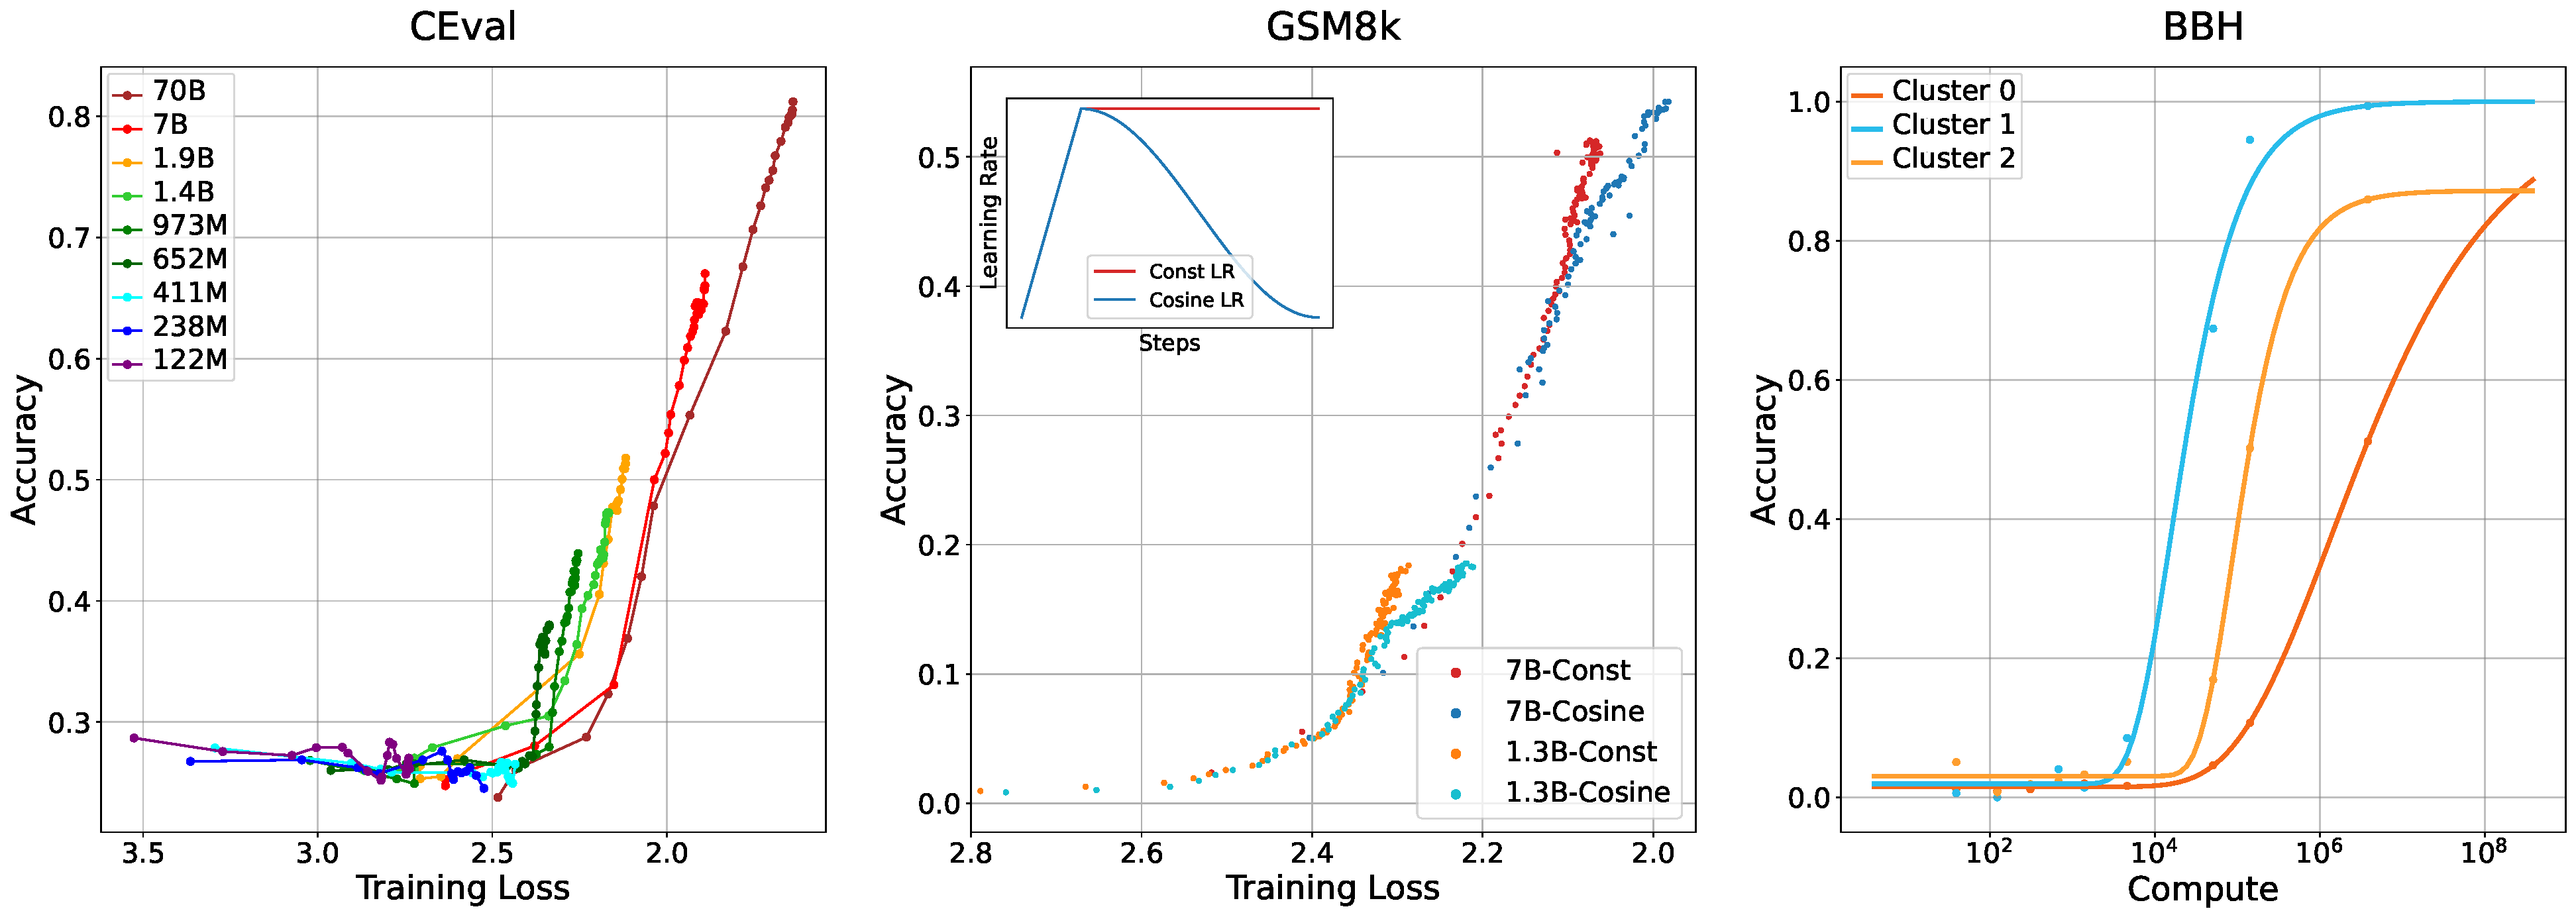
\includegraphics[width=\linewidth]{figures/related_works/ff_gsm8k_cot_v1_avg_score_loss_perf.pdf}
    \caption{Performance-loss relationship across different model sizes (left) and learning rate schedules (middle). Performance-compute relationship for different clusters of the BBH samples(right)}
    \label{fig:perf-loss}
    \vspace{-14pt}
\end{figure*}
In this section, we present the pilot experiments to illustrate the shortcomings of existing approaches. 

\noindent\textbf{Training loss may mismatch downstream task performance.}
Predicting downstream performance from training loss assumes LLMs achieve identical downstream results at the same loss value, which does not hold universally.
%
In practice, training loss primarily serves as an indicator of in-domain fitting, whereas downstream tasks typically represent out-of-domain evaluations. Moreover, training configurations, such as model size and learning rate, can significantly affect not only the final loss but also the model’s generalization capabilities.


\cref{fig:perf-loss}(left) illustrates the performance–loss relationships for LLMs of different sizes on the CEval benchmark~\citep{nguyen2024ceval}. At the same training loss level, smaller models can outperform larger ones in terms of test accuracy. Because smaller models initially exhibit weaker in-domain fitting capacity, they typically require more training steps to reach the same loss value, which can lead to better in-domain generalization once they do. \cref{fig:perf-loss}(middle) compares the performance of LLMs trained under different learning rate schedules on the GSM8k dataset~\citep{cobbe2021training}. At the same loss level, the performance under the cosine schedule is always worse than that under the constant schedule, indicating that a lower learning rate may prioritize memorization over generalization, thereby diminishing downstream performance.

\noindent\textbf{Diverse scaling patterns within the evaluation set.}
Different task samples exhibit unique computational thresholds, learning slopes, and upper bounds, making it challenging to find a single fitting function (or function group) that generalizes well across diverse task samples. \cref{fig:perf-loss}(right) illustrates the performance-compute relationships \revise{on three clusters randomly selected from those formed by clustering tasks based on their difficulty in the BBH benchmark.}~\citep{suzgun2023challenging}, with each cluster containing samples with similar difficulty. Even within a single evaluation set, these scaling curves can vary significantly, indicating that a one-size-fits-all performance-compute curve is insufficient for capturing the full spectrum of a downstream evaluation set.

Taken together, these observations highlight the importance of modeling the heterogeneous scaling properties within an evaluation set and identifying a robust intermediate metric to serve as a reliable indicator of the downstream performance of LLMs.
% \begin{figure*}[t]
%   \includegraphics[width=0.48\linewidth]{example-image-a} \hfill
%   \includegraphics[width=0.48\linewidth]{example-image-b}
%   \caption {A minimal working example to demonstrate how to place
%     two images side-by-side.}
% \end{figure*}

\begin{figure*}[t]
    \centering
    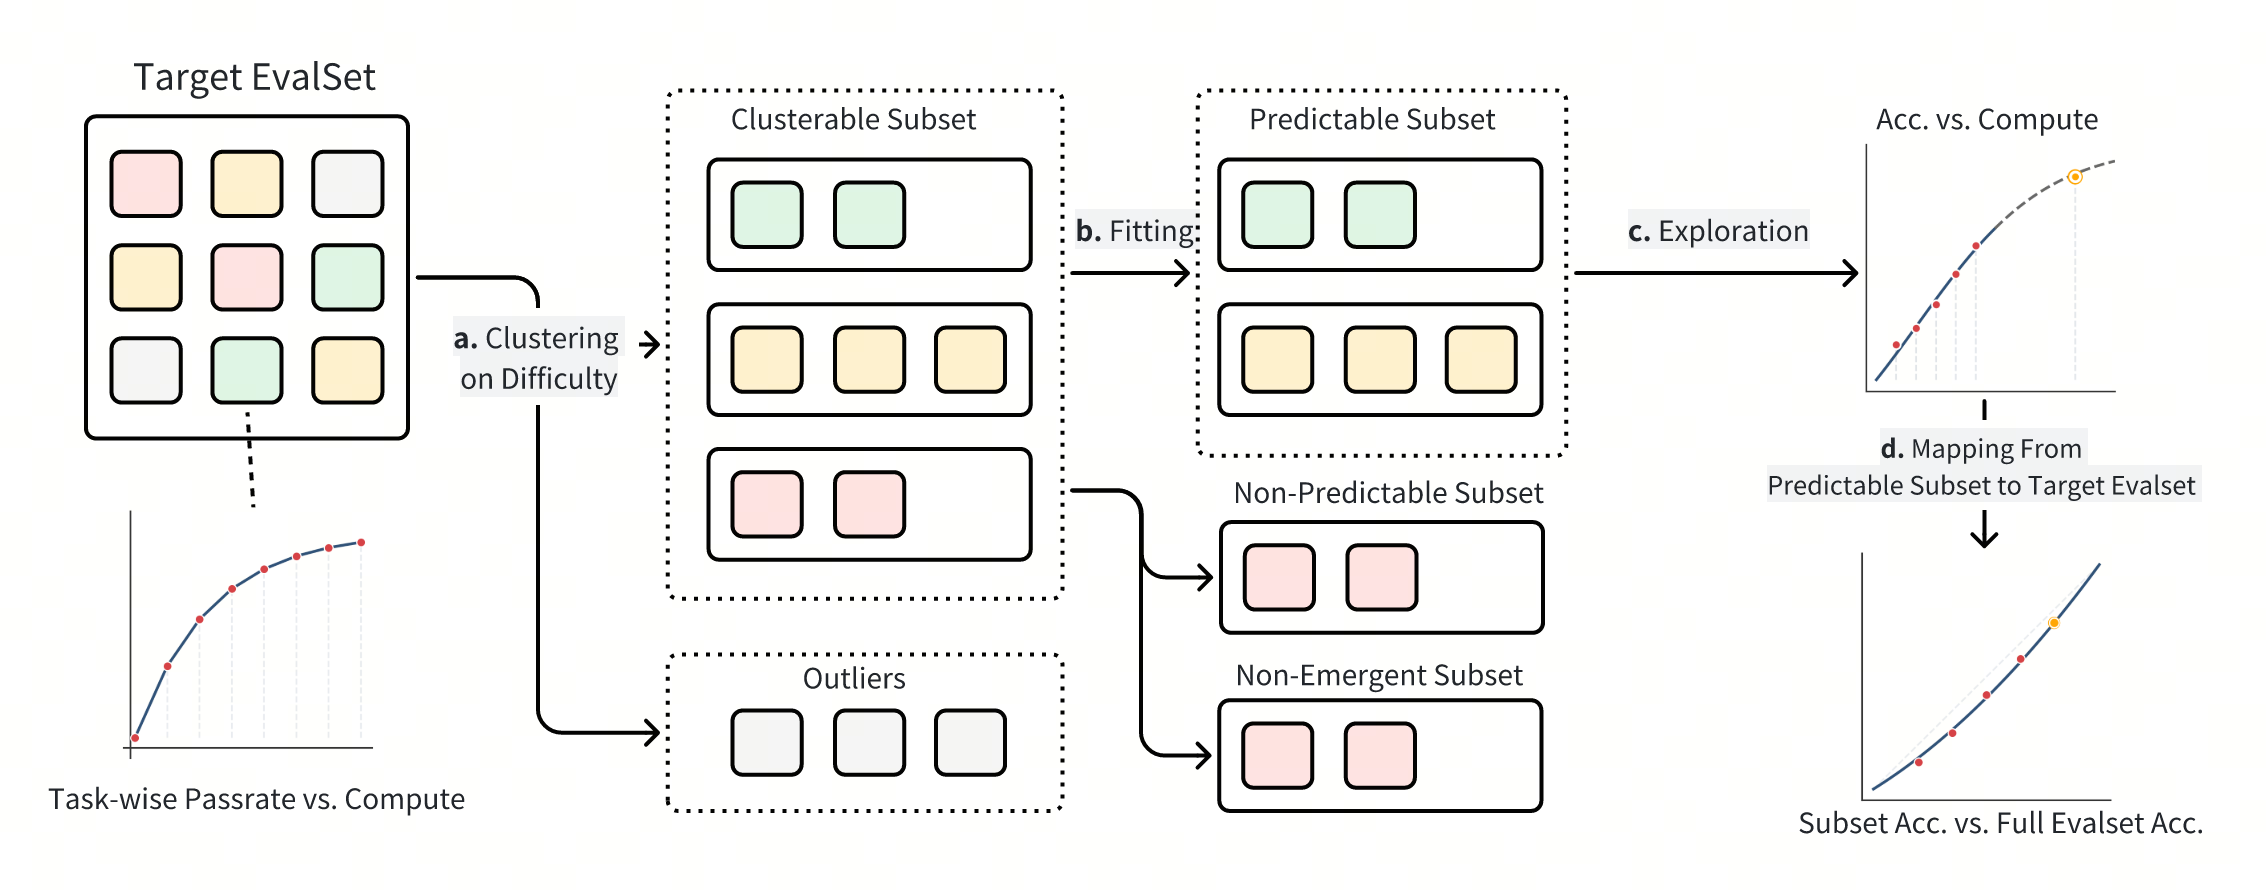
\includegraphics[width=\linewidth]{figures/method/MainPipeline.png}
    \vspace{-15pt}
    \caption{The pipeline of Cluster-On-Difficulty downstream task performance scaling, including 4 stages: \textbf{a}. Represent task difficulty feature with task-wise passrate vector. Cluster on the difficulty feature and filter outliers. \textbf{b}. Fit cluster-wise performance-compute curve. Classify clusters into extrapolatable clusters, non-extrapolatable clusters, and non-emergent clusters. \textbf{c}. Predict accuracy on extrapolatable clusters. \textbf{d}. Map subset accuracy prediction to full evaluation set performance.}
    \label{fig:main-pipeline}
    \vspace{-7.5pt}
\end{figure*}

